\section{Methodology and Data}
\label{sec:method}

\subsection{The Nelson-Siegel model}
\label{sec:n-s_model}

This section is aimed at outlining the methodology applied in this thesis. After giving a comprehensive primer on the aforementioned model of the yield curve established by \citet{nelson1987parsimonious}, the identification strategy for the VAR model containing macroeconomic and yield curve variables is introduced.

The first step of the two-step methodological approach involves modelling the yield curve using the Nelson-Siegel three factor model. 
The genius of the Nelson-Siegel decomposition lies within its flexibility as well as its parsimony. 
Based on a set of observable yields, the model is able to capture a wide range of yield curve shapes in a rather simplistic manner by decomposing the entire term structure solely into three factors.
Another core strength is its ability to enable analysts to inter- and extrapolate between yields within the sample, thus providing yields for all maturities along the curve.
As mentioned in section \ref{sec:lit_rev}, the Nelson-Siegel model performs relatively well in out-of sample forecasting.
What is more, though it does not explicitly ensure the absence of arbitrage, \citet{coroneo2011arbitrage} show that the Nelson-Siegel model aligns with the assumption of no-arbitrage. 
Given these highly promising attributes, the Nelson-Siegel approach appears to be well suited for the task at hand.

Following the representation of \citet{diebold2006macroeconomy}, while also leaning on the foundational work provided by \citet{diebold2006forecasting}, the yield curve at any time $t$ is thus assumed to be represented as the \citet{nelson1987parsimonious} model:

% Thus, the estimated\footnote{The estimation of the yield curve factors is conducted using the Nelson.Siegel method from the R package \href{https://cran.r-project.org/web/packages/YieldCurve/index.html}{YieldCurve}} model of the yield curve used in this thesis is represented by:

\usetagform{default}
\begin{equation}
\label{eq:NS_factor_interpretation}
    y_{t}(\tau)=L_{t}+S_{t}\left(\frac{1-\mathrm{e}^{-\lambda \tau}}{\lambda \tau}\right)+C_{t}\left(\frac{1-\mathrm{e}^{-\lambda \tau}}{\lambda \tau}-\mathrm{e}^{-\lambda \tau}\right) + \varepsilon_{t},
\end{equation}

where $t=1,\ldots, T$, $y_{t}(\tau)$ is a set of $N$ yields, each with a distinct maturity $\tau$, used for the decomposition, $L_{t}$, $S_{t}$, $C_{t}$ and $\lambda$ are the parameters to be estimated, while $\varepsilon_{t}$ represents the error term.
The regressors, which are also known as the factor loadings, are central for ensuring the flexibility to represent various yield curve shapes, where $\lambda$ shows their respective rate of decay.
The loading on  $L_{t}$ is 1 for all maturities,
%and is thus, interpreted as the long-term factor
while the loading on the second factor,  $S_{t}$ starts at 1 and decays monotonically towards 0.
%, and thus can be viewed as a short-term factor. 
Finally, the loading on the third factor,  $C_{t}$, starts at 0, increases, but then decays back to 0.
The significance of the $\lambda$ coefficient can be seen in Figure \ref{fig:factor_loadings_lambdas}, illustrating the factor loadings given a set of two different values for the rate of decay.
While the level factor is 1 regardless of $\lambda$, it is evident that a higher $\lambda$ implies a faster decay towards 0 of the slope and curvature factor loading. 
As a result, the lower the estimated $\lambda$ coefficient, the higher the loading induced by yields at longer maturities for both the slope and the curvature factor. 
Moreover, $\lambda$ determines where the loading on $C_{t}$ reaches its maximum, where a lower rate of decay implies a maximum at a relatively longer maturity. 
In this context, Figure \ref{fig:factor_loadings} offers a concrete example showing the US Treasury yield curve as of December 2019 based on data provided by \citet{liu2021reconstructing} along with the estimated factor loadings. 
One can see that the yield curve is upward sloping, though there is a clear hump at the short as well as the long-end end.
The long-term factor is one regardless of the maturity.
The slope factor is (per definition) at its maximum at the 1-month maturity, decreasing exponentially with increasing maturity, and hence having the highest loadings at the short-end.  
The medium-term factor is increasing, reaching --- rather prematurely --- its maximum around the 14-month maturity, after which it is decreasing towards 0.

As shown by \citet{diebold2006forecasting}, the regression coefficients can have economically meaningful interpretations, i.e. they are the time-varying level ($L_{t}$), slope 
%
($S_{t}$)\footnote{As shown by \citet{diebold2006forecasting}, $S_{t}$ equals the negative slope, that is, the difference between short-term and long-term yields} 
%
and curvature ($C_{t}$) factors, respectively. 
% , where $\lambda$ shows the rate of decay of each individual factor loading.
What is more, $L_{t}$ can be thought of as the long-term factor since the loading is identical for all maturities, implying that an increase in the level factor increases all yields across the entire yield curve.
%in a term structure setting represented by equation \ref{eq:NS_factor_interpretation}.
%, hence governing the overall level of yields. 
By contrast, the slope factor is interpreted as the short-term factor since short-term rates induce a heavier loading on  $S_{t}$, thereby changing the slope of the yield curve.
Similarly, the curvature factor is considered as the medium-term component since medium-term yields tend to have the highest loading, while simultaneously an increase in $C_{t}$ will mainly increase medium-term yields.
%\citep{diebold2006forecasting}.
%, hence, it may be thought of as the medium-term factor. 
The contribution of each factor loading to the overall shape of the estimated yield curve is thus given by each respective factor, e.g.  $L_{t}$ shows the contribution of the long-term factor,  $S_{t}$ that of the short-term component, while  $C_{t}$ illustrates the contribution of the medium-term component \citep{nelson1987parsimonious}.


% \usetagform{fn}
% \begin{equation}
% \label{eq:NS_basic}
%     y_{t}(\tau)=\beta_{1t}+\beta_{2t}\left(\frac{1-\mathrm{e}^{-\lambda \tau}}{\lambda \tau}\right)+\beta_{3t}\left(\frac{1-\mathrm{e}^{-\lambda \tau}}{\lambda \tau}-\mathrm{e}^{-\lambda \tau}\right),
% \end{equation}
% \footnotetext{Mathematically, this representation can be thought of as a constant plus a Laguerre function \citep{nelson1987parsimonious}}

\begin{figure}[t]
    \centering
    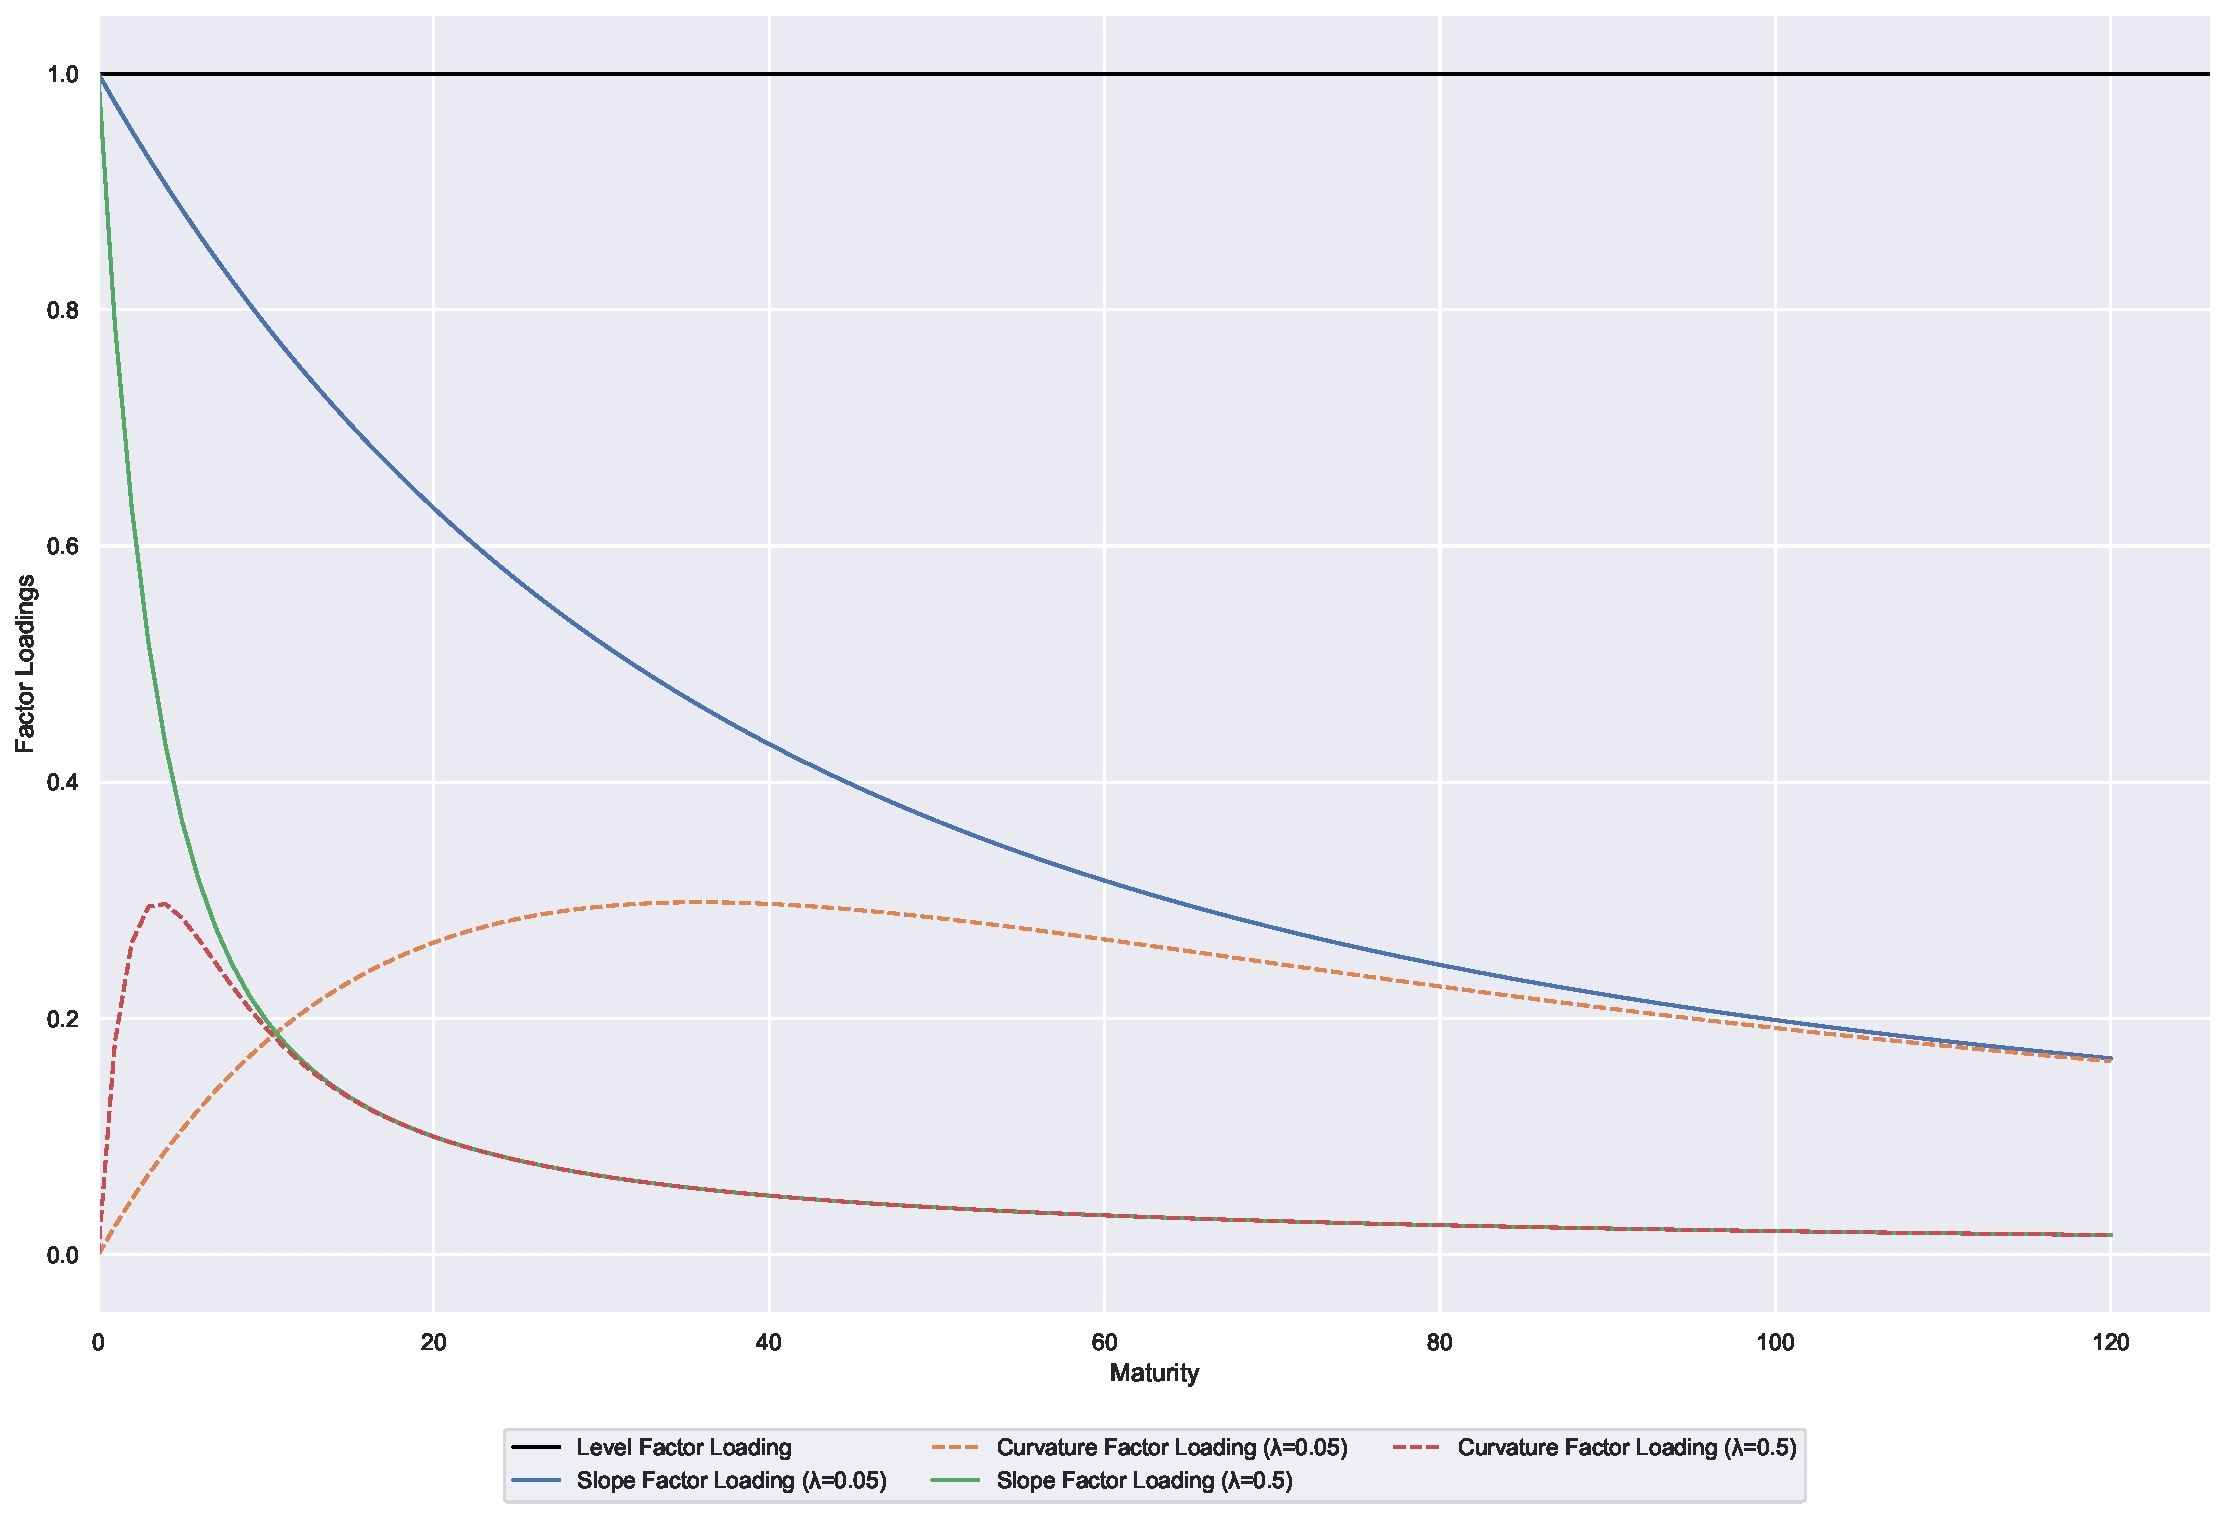
\includegraphics[width=15cm]{Figures/Factor_Loadings_Lambdas.pdf}
    \caption{Exemplary Nelson Siegel Factor Loadings}
    \label{fig:factor_loadings_lambdas}
    
\end{figure}

As described in \citet{nelson1987parsimonious}, the estimation\footnote{The estimation of the yield curve factors in this thesis is conducted using the Nelson.Siegel method from the R package \href{https://cran.r-project.org/web/packages/YieldCurve/index.html}{YieldCurve}} can be conducted in the following way. For a provisional value $\lambda$, the sample values for the factor loadings are calculated. Based thereupon, the best-fitting yield curve factors are estimated using ordinary least squares (OLS). This procedure is repeated over a grid of values for $\lambda$, yielding the overall best-fitting values for $\lambda$, $L_{t}$, $S_{t}$, and $C_{t}$. 
Alternatively, $\lambda$ can be chosen beforehand after which the best fitting Nelson-Siegel factors are estimated based on the imposed loadings at a specific maturity.
As done by \citet{Fischer_et_al_2023} --- based on the work by \citet{diebold2006forecasting} --- the estimation of the three yield curve factors in this thesis is implemented by setting the rate of decay to $\lambda = 0.7308$ and fitting the Nelson-Siegel model to the prevailing yield curve for each time period $t$ in the sample, resulting in the best fitting a level ($L_{t}$), slope ($S_{t}$) and curvature ($C_{t}$) factors, respectively.
%, i.e., the zero-coupon yields contained in vector $y_{t}$ at different maturities $\tau_{N}$. 
Consequently, these factors are assumed to be an approximate representation of the yield curve at any given time $t$ ---dramatically reducing the dimensionality compared to including each yield separately --- and, together with the macroeconomic variables, are included in a VAR(p) model aimed at studying the link between the economy and the yield curve. 
% In a more comprehensive matrix representation, the estimation of the factors is done using the following system of linear equations, where each row corresponds to equation \ref{eq:NS_factor_interpretation} with a specific yield $y_{t}$ and a corresponding maturity $\tau_{N}$ as well as an error term $\varepsilon_{t}(\tau_{N})$:

% \usetagform{fn}
% \begin{equation}
% \left(\begin{array}{c}
% y_t\left(\tau_1\right) \\
% y_t\left(\tau_2\right) \\
% \vdots \\
% y_t\left(\tau_N\right)
% \end{array}\right)=\left(\begin{array}{ccc}
% 1 & \frac{1-\mathrm{e}^{-\tau_1 \lambda}}{\tau_1 \lambda} & \frac{1-\mathrm{e}^{-\tau_1 \lambda}}{\tau_1 \lambda}-\mathrm{e}^{-\tau_1 \lambda} \\
% 1 & \frac{1-\mathrm{e}^{-\tau_2 \lambda}}{\tau_2 \lambda} & \frac{1-\mathrm{e}^{-\tau_2 \lambda}}{\tau_2 \lambda}-\mathrm{e}^{-\tau_2 \lambda} \\
% \vdots & \vdots & \vdots \\
% 1 & \frac{1-\mathrm{e}^{-\tau_N \lambda}}{\tau_N \lambda} & \frac{1-\mathrm{e}^{-\tau_N \lambda}}{\tau_N \lambda}-\mathrm{e}^{-\tau_N \lambda}
% \end{array}\right)\left(\begin{array}{c}
% L_t \\
% S_t \\
% C_t
% \end{array}\right)+\left(\begin{array}{c}
% \varepsilon_t\left(\tau_1\right) \\
% \varepsilon_t\left(\tau_2\right) \\
% \vdots \\
% \varepsilon_t\left(\tau_N\right)
% \end{array}\right)
% \end{equation}
% \footnotetext{This corresponds to the measurement equation in \citet{diebold2006macroeconomy}}






\begin{figure}[t]
    \centering
    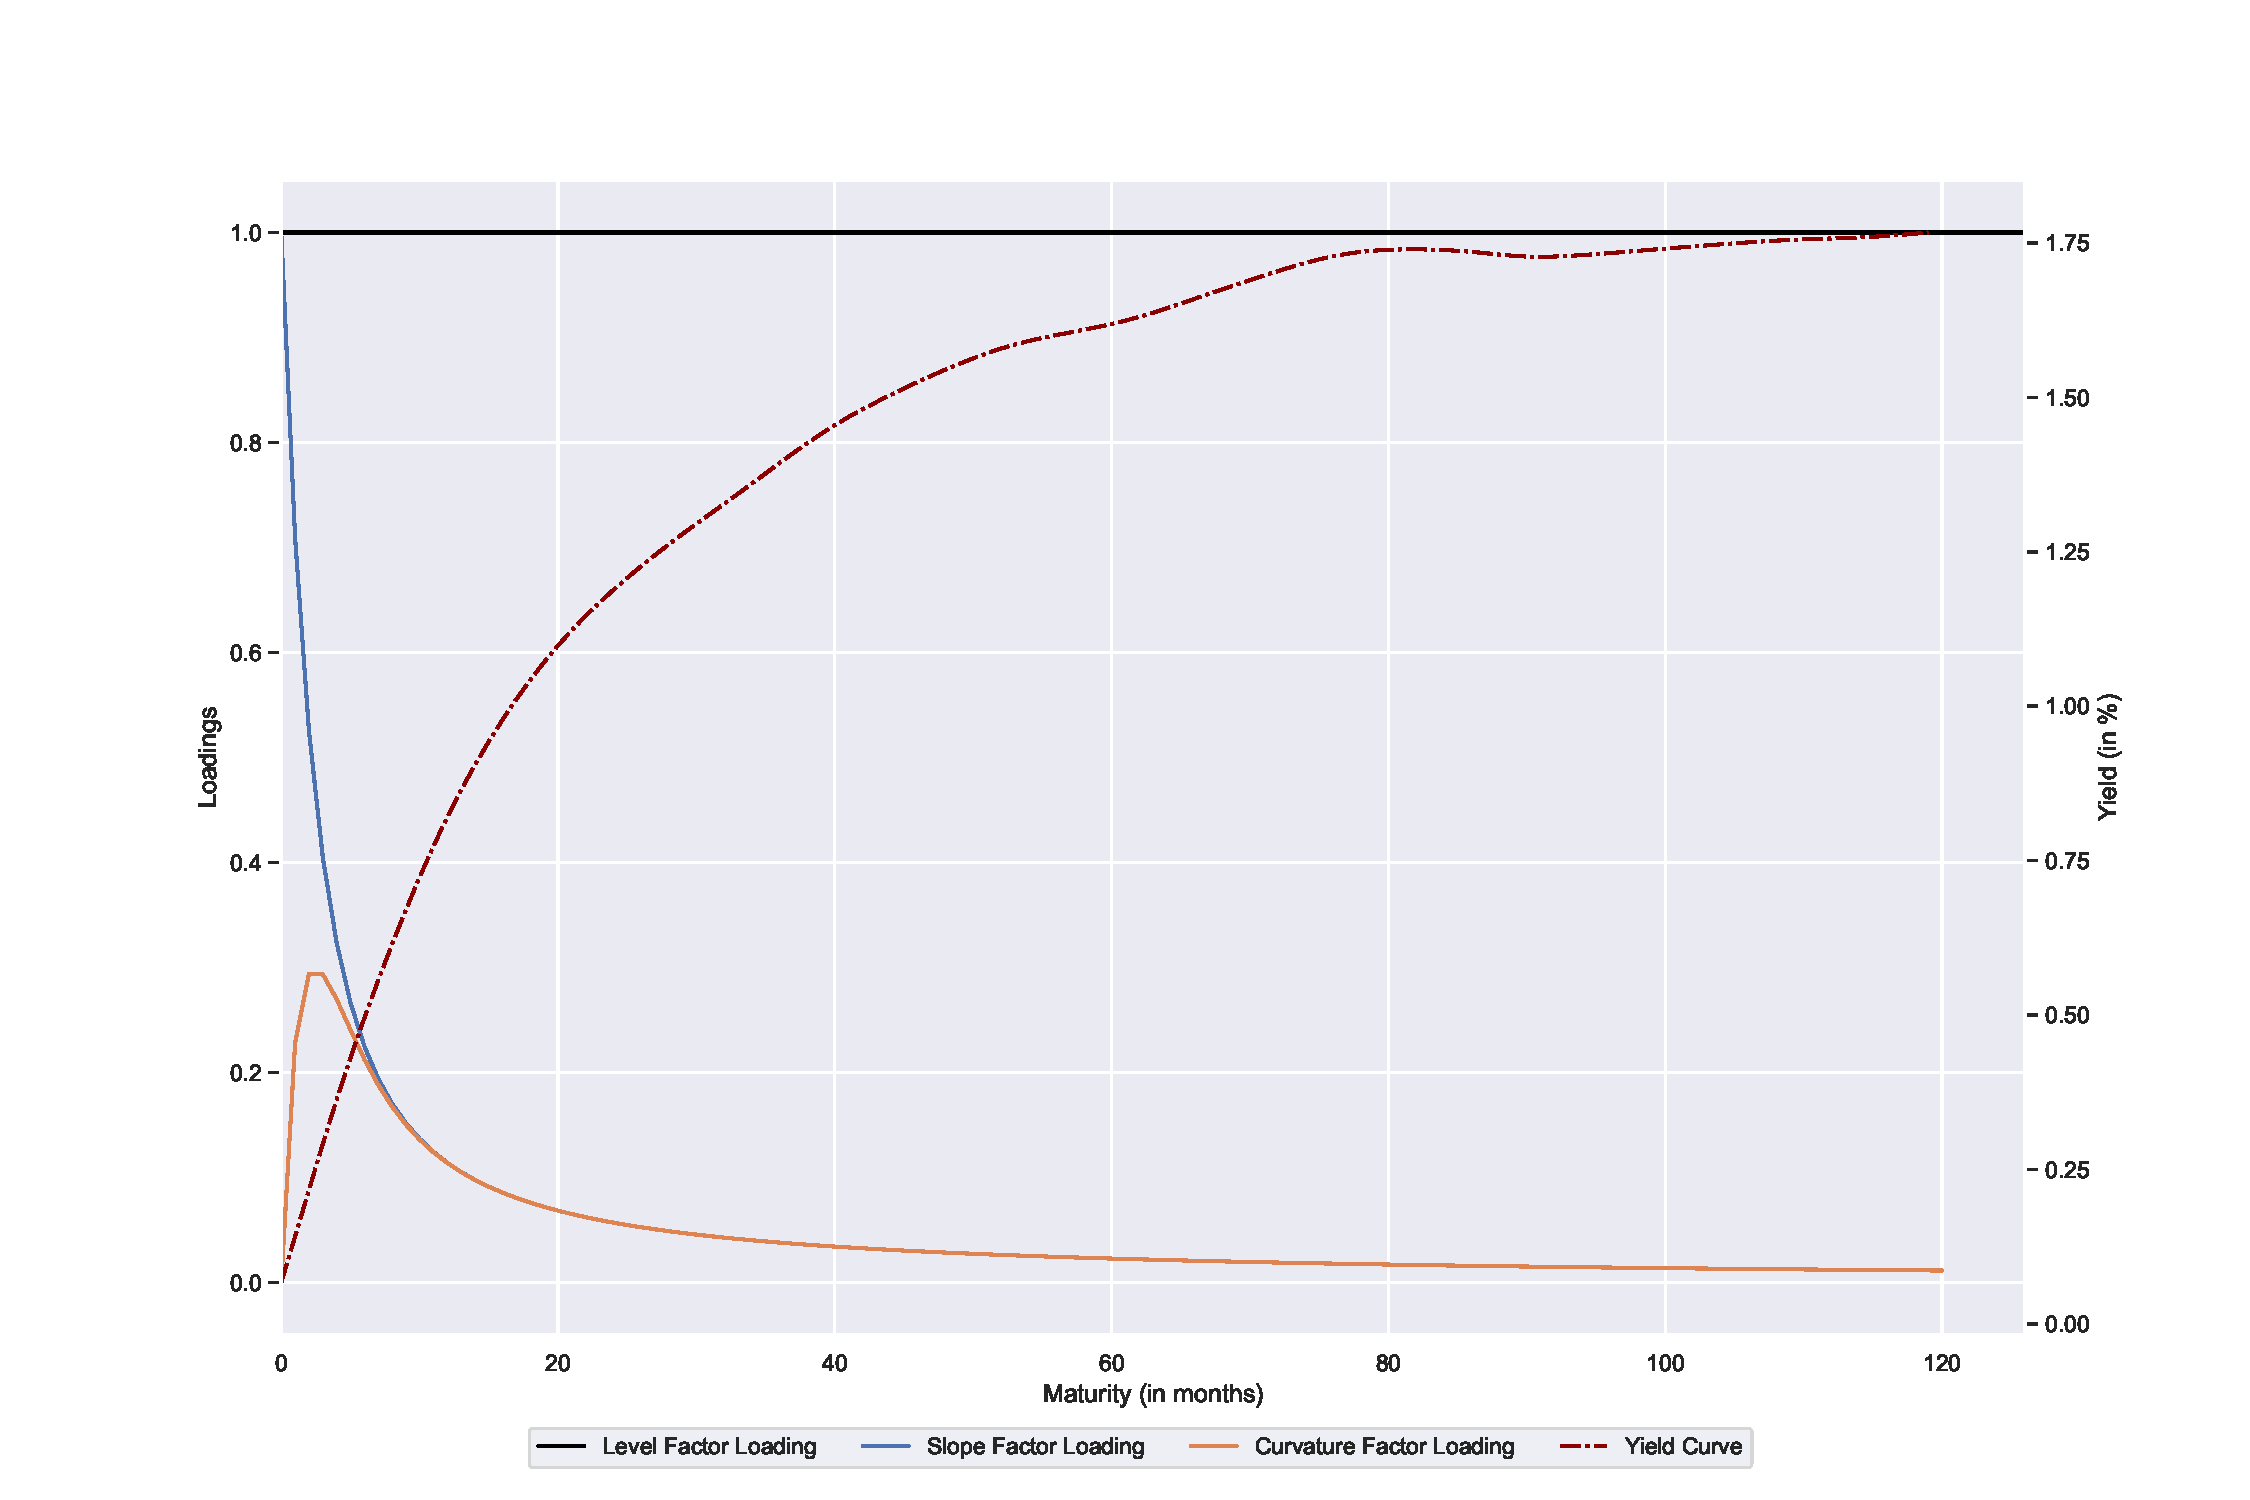
\includegraphics[width=15cm]{Figures/Factor_Loadings_Plot.pdf}
    \caption{Actual Nelson Siegel Factor Loadings}
    \label{fig:factor_loadings}

    \begin{minipage}{.7\linewidth}
    \footnotesize
    \medskip
    \emph{Note:} This figure provides a graphical illustration of the Nelson Siegel factor loadings based on the US Treasury yield curve as of January 2022 ($\lambda = 0.7308$).
    \end{minipage}
    
\end{figure}




\subsection{Vector autoregression}

% \textbf{VAR description + variable ordering $\Rightarrow$ ecbwp1276}

Aforesaid VAR(p) model forms the second step of the analysis and --- ignoring the vector containing the intercept terms $c$ --- is represented in the following way:
% After the extraction of the three factors, the corresponding time series of the factors are included in a 
\usetagform{default}
\begin{equation}
\bm{Y}_{t}=\sum_{p=1}^p 
\bm{A}_{p} \mathbf{Y}_{t-p}+\bm{\varepsilon}_{t}, \ \bm{\varepsilon}_{t} \sim \mathcal{N}\left(0, \bm{\Sigma_{\varepsilon}}\right),
\end{equation}
where $Y_{t}$ denotes the $(K \times 1)$ matrix containing $K$ endogenous variables, $c$ is a $(K \times 1)$ vector of intercept terms, $p$ denotes the maximum lag length, $A_{p}$ is a $(K \times K)$ matrix of the autoregressive coefficients for lag length $p$ and $\varepsilon_{t}$ is a $(K \times 1)$ matrix of the reduced-form error terms. 

The identification strategy is based on a structural VAR approach using contemporary recursive restrictions via a Cholesky decomposition of the variance-covariance matrix of the reduced-form errors $\Sigma_{\varepsilon}$. Largely following the notation of \citet{kilian2017structural}, the representation of the structural VAR --- again ignoring the intercept vector $c$ --- as well as the relationship between the reduced-form and structural form VAR can be seen by:

\usetagform{default}
\begin{equation}
\label{eq:structural_VAR}
    \begin{split}
   \bm{B}_{0}\bm{Y}_{t}= \bm{B}_{p} \bm{Y}_{t-p}+\bm{\omega}_{t}, \ \bm{\omega}_{t} \sim \mathcal{N}\left(0, \bm{I}\right), \\
   \\
    \underbrace{\bm{B}^{-1}_{0}\bm{B}_{0}}_{\bm{I}}\bm{Y}_{t}= \underbrace{\bm{B}^{-1}_{0}\bm{B}_{p}}_{\bm{A}_{p}} \bm{Y}_{t-p}+\underbrace{\bm{B}^{-1}_{0}\bm{\omega}_{t}}_{\bm{\varepsilon}_{t}},
    \end{split} 
\end{equation}

% \textbf{explain in more detail $B^{-1}_{0}$ and the aim of the VAR(p) identification strategy}

% where the crucial ... $B_{0}$.
where $\omega_{t}$ is the serially uncorrelated vector of the structural shocks.
Since these structural shocks permit to deduce causal conclusions based on the correlations within the data, the central aim of this thesis is the identification of the structural shocks, whereupon the relationship between the model variables are examined. 
As can be seen in equation \ref{eq:structural_VAR}, identification depends upon identifying the inverse of matrix $B_{0}$, which governs the contemporaneous relationship between the model variables.
In this thesis, it is obtained applying the aforementioned Cholesky decomposition of the variance-covariance matrix of the reduced-form errors. 
$B^{-1}_{0}$ shows how each (correlated) reduced-form shock is a linear combination of specific (uncorrelated) structural shocks. 
To be precise, $B^{-1}_{0}$ is a lower-triangular matrix, where each element above the main diagonal is zero, and it depicts how a structural shock to each variable affects each of the models variables on impact, thus allowing for the inference of potential relationships among the variables in the model. 
Since the identification of $B^{-1}_{0}$ is not unique with respect to the ordering of the variables, assessing the economic adequacy of the chosen ordering is crucial. 
In particular, as all elements above the main diagonal are zero, implying that one assumes that the variables ordered first tend to be affected by the other variables with a delay of at least one period, it would generally be reasonable to order the variables from the slowest to the fastest reacting. 
% In particular, as each column of $B^{-1}_{0}$ shows how each structural shock contemporaneously affects all endogenous variables in the model, and since all elements above the main diagonal are zero, implying that one assumes that some variables tend not to be affect by the other variables with a delay of at least one period, it would be reasonable to 
In summary, following the estimation of a VAR(p) model containing specific macroeconomic and yield curve variables and applying the identification strategy described above, the orthogonal shocks, based on a certain variable ordering, are used to identify the relationship between the macroeconomy and the yield curve. 



% \begin{equation}
% \underbrace{\left[\begin{array}{c}
% \varepsilon_t^{\tilde{y}} \\
% \varepsilon_t^\pi \\
% \varepsilon_t^i
% \end{array}\right]}_{\boldsymbol{\varepsilon}_{\boldsymbol{t}}}=\underbrace{\left[\begin{array}{lll}
% b_0^{11} & b_0^{12} & b_0^{13} \\
% b_0^{21} & b_0^{22} & b_0^{23} \\
% b_0^{31} & b_0^{32} & b_0^{33}
% \end{array}\right]}_{\boldsymbol{B}_0^{-1}} \underbrace{\left[\begin{array}{c}
% e_t^{\tilde{y}} \\
% e_t^\pi \\
% e_t^i
% \end{array}\right]}_{\boldsymbol{e}_{\boldsymbol{t}}}
% \end{equation}

Based on a standard identification set proposed by the likes of \citet{Furlanetto_2017}, the empirical analysis presented in section \ref{sec:analysis} is conducted using $K=8$ variables, where the relevant macroeconomic variables are industrial production ($IP_t$), inflation ($\pi_t$), and a short-term interest rate ($i_t$), while the financial variables include an indicator for financial stress ($FS_t$) and a variable representing the stock market ($M_t$). 
The variables representing the yield curve are the three factors obtained from the first step via the Nelson-Siegel decomposition ($L_t, S_t, C_t$). 
Drawing from \citet{martins2010level}, who argue that financial variables may more prone to be affected instantaneously by shocks to the macroeconomy while the latter may react more slowly to shocks to the former, the variables are ordered from the most exogenous to the least exogenous. Thus, the ordering of vector $Y_{t}$ is given by
$Y_{t} = [IP_{t}, \ \pi_{t}, \ i_{t}, \ FS_{t}, \ L_{t}, \ S_{t}, \ C_{t}, \ M_{t}]$.
% $
% % $\left[ 
% % \begin{array}{cccccccc}
% %      IP_{t}, &  \pi_{t}, & i_{t}, & FS_{t}, & L_{t}, & S_{t}, & C_{t}, & M_{t} 
% % \end{array}
% \right]$.
This ordering is also consistent with, among others, \citet{ang2003no}, who order their macro variables before the included yields in their VAR approach. 
While the macroeconomic variables being ordered first appears plausible given the fact that they often tend to react in a lagged manner, the stock market being ordered last broadly follows \citet{kilian2009impact}, assuming that the stock market reacts to shocks to the other variables contemporaneously, which seems reasonable as it is generally assumed 
% that stock prices encompass all relevant information at any time $t$ and 
that stocks instantaneously incorporate any new information available,\footnote{See, for example, \citet{pearce1984stock, beaudry2006stock, ormos2011impacts} for a discussion about the response of stock prices to economic news} while, following the previously mentioned assumption that macro variables tend to react inertly, it does affect all other variables only with a delay of at least one period.


% \textbf{RESEARCH and CITE papers that show that macro variables react slowly and stock market reacts instantaneously!!!}

% \textbf{Structural VAR form $\Rightarrow$ Kilian, Park (2009), p. 4 ff}

% \textbf{SHOW Cholesky decomposition as identification strategy}. 

% After the estimation of the VAR(p) model, the orthogonal shocks are used to identify the relationship between the macroeconomy and the yield curve. They can be represented in the following way:

% \begin{equation}
% \left(\begin{array}{l}
% u_t^p \\
% u_t^{g d p} \\
% u_t^m \\
% u_t^i \\
% u_t \\
% u_t \\
% u_t \\
% u_t
% \end{array}\right)=\left[\begin{array}{cccccccc}
% b_0^{11} & 0 & 0 & 0 & 0 & 0 & 0 & 0\\
% b_0^{21} & b_0^{22} & 0 & 0  & 0 & 0 & 0 & 0\\
% b_0^{31} & b_0^{32} & b_0^{33} & 0 & 0 & 0 & 0 & 0\\
% b_0^{41} & b_0^{42} & b_0^{43} & b_0^{44} & 0 & 0 & 0 & 0 \\
% b_0^{41} & b_0^{42} & b_0^{43} & b_0^{44} & 0 & 0 & 0 & 0 \\
% b_0^{41} & b_0^{42} & b_0^{43} & b_0^{44} & 0 & 0 & 0 & 0 \\
% b_0^{41} & b_0^{42} & b_0^{43} & b_0^{44} & 0 & 0 & 0 & 0 \\
% b_0^{41} & b_0^{42} & b_0^{43} & b_0^{44} & 0 & 0 & 0 & 0 \\
% \end{array}\right]\left(\begin{array}{l}
% w_{1 t} \\
% w_{2 t} \\
% w_{3 t} \\
% w_{4 t} \\
% w_{5 t} \\
% w_{6 t} \\
% w_{7 t} \\
% w_{8 t} \\

% \end{array}\right)
% \end{equation}

% \usetagform{default}
% \begin{equation}
%     \left(\begin{array}{c}
% L_t-\mu_L \\
% S_t-\mu_S \\
% C_t-\mu_C
% \end{array}\right)=\left(\begin{array}{lll}
% a_{11} & a_{12} & a_{13} \\
% a_{21} & a_{22} & a_{23} \\
% a_{31} & a_{32} & a_{33}
% \end{array}\right)\left(\begin{array}{c}
% L_{t-1}-\mu_L \\
% S_{t-1}-\mu_S \\
% C_{t-1}-\mu_C
% \end{array}\right)+\left(\begin{array}{c}
% \eta_t(L) \\
% \eta_t(S) \\
% \eta_t(C)
% \end{array}\right),
% \end{equation}

Though the selected methodology applied in the thesis has, in various forms and alterations, been applied quite often in the literature, a tremendous amount of alternative approaches is available in the economist's toolbox. 
A comprehensive overview of these numerous potential methodological approaches modelling the yield curve and studying it's relationship with the macroeconomy is offered in \citet{diebold2013yield}. 
